\documentclass[12pt]{article}
\usepackage[left=2cm, top=2cm, right=2cm, bottom=2cm]{geometry}
\usepackage[utf8]{inputenc}
\usepackage[T1]{fontenc}
\usepackage[french]{babel}
\usepackage{graphicx}
\usepackage{graphics}
\usepackage{amsmath}
\usepackage{tikz}
\usepackage{graphicx}
\usepackage{xcolor}
\usepackage{parskip}
\usepackage{physics}
\usepackage{tikz}


\title{\textbf{Méthodes expérimentales} \\ TP 4: Étude des propriétés thermodynamiques d'un gaz presque parfait}
\author{MENARD Alexandre \\ VIEILLEDENT Florent}

\setlength{\parindent}{1cm}

\begin{document}
\maketitle

\section*{Introduction}
Dans ce travail pratique, on cherchera à vérifier la loi des gaz parfaits. Le gaz utilisé sera l'air qu'on considère ici comme un gaz parfait. Dans un premier temps, on mesurera la pression d'un gaz en faisant varier le volume de ce gaz avec une température constante. On utilisera pour cela une seringue et un pressiomètre Jeulin. 
On mesurera ensuite la pression d'un gaz à volume constant en faisant varier la température. On utilise pour ça une bouteille étanche et un manomètre.

\newpage
\section{Relation entre le volume et la pression à température donnée}

Dans cette première expérience on cherche à vérifier que le produit PV est une constante. Pour cela, on calcule la pression d'un gaz pour différentes valeurs de volume, sans changer la température. 	

\subsection{Expérimentation}

La seringue est placé initialement sur $15\, cm^3$. On relie ensuite la seringue au pressiomètre Jeulin gràce à un tuyau. On fait varier le volume de la seringue et on note la pression donnée par le pressiomètre. 

\begin{figure}[!h]
	\begin{center}
		\includegraphics[scale=0.2]{Schéma_seringue.png}
		\label{Schéma_seringue}
		\caption{Schéma de la première expérience avec la seringue et le pressiomètre}
	\end{center}
\end{figure}




On note $V_{seringue}$ le volume à l'intérieur de la seringue. On fait varier ce volume de $15\, cm^3$ à $60\, cm^3$ tout les $5\, cm^3$. La seringue est graduée tout les $cm^3$, donc notre incertitude sur le volume est $\delta V_{seringue}=0.5 \, cm^3$.  On note pour chaque volume la pression donnée par le pressiomètre. L'incertitude sur le pressiomètre est de $2\% $. On a donc $\delta P = 0.02*P$. On répète les mesures 3 fois pour avoir une meilleur estimation de l'incertitude. On note respectivement P1,P2 et P3 les mesures de pressions lors de la première, deuxième et troisième mesure. 

\begin{figure}[!h]
	\begin{center}
		\includegraphics[scale=0.04]{img/exp1.png}
		\label{Photo exp1}
		\caption{Montage de la première expérience}
	\end{center}
\end{figure}
\newpage
On regroupe nos données dans un tableau.
\begin{table}[h!]
	\begin{center}
		\begin{tabular}{|c|c|c|c|c|c|c|}	
\hline
 $V_{seringue} (cm^3)$ &  $P1 (hPa)$ &  $\delta P1(hPa)$ &  $P2 (hPa)$ &  $\delta P2(hPa)$ &  $P3 (hPa)$ &  $\delta P3(hPa)$ \\
\hline
            15 &              1003 &            20 &              1050 &            21 &              1070 &            21 \\
            20 &               792 &            16 &               810 &            16 &               816 &            16 \\
            25 &               640 &            13 &               654 &            13 &               652 &            13 \\
            30 &               542 &            11 &               552 &            11 &               556 &            11 \\
            35 &               468 &             9 &               474 &             9 &               480 &            10 \\
            40 &               410 &             8 &               417 &             8 &               427 &             9 \\
            45 &               368 &             7 &               374 &             7 &               374 &             7 \\
            50 &               331 &             7 &               337 &             7 &               338 &             7 \\
            55 &               302 &             6 &               304 &             6 &               308 &             6 \\
            60 &               276 &             6 &               283 &             6 &               284 &             6 \\
\hline
		\end{tabular}
	\end{center}
	\label{Tableau première expérience}
	\caption{Tableau des données de la première expérience}
\end{table}



\subsection{Modélisation}

On rappel la loi des gaz parfait, avec R la constante des gaz parfaits,P la pression du gaz, V son volume et T sa température:
\begin{equation}
PV=nRT
\end{equation}

Nous devrions donc obtenir une droite si nous traçons P en fonction de $\frac{1}{V}$, car on a $P=\frac{a}{V}$ avec $a=nRT$.  

Dans un premier temps, on prend $V=V_{seringue}$. D'après la méthode de la dérivée, l'incertitude associée est:
\begin{equation}
\delta \frac{1}{V_{seringue}}=\frac{1}{V_{seringue}^2}*\delta V_{seringue}
\end{equation}

Pour la pression, on effectue la moyenne des 3 pressions mesurées. On a :
\begin{equation}
P=\frac{P1+P2+P3}{3}
\end{equation}

En effectuant les dérivées partielles, on trouve l'incertitude sur la pression:
\begin{align*}
\delta P &= \abs{\frac{\partial P}{\partial P1}} \delta P1 +\abs{\frac{\partial P}{\partial P2}} \delta P2 +\abs{\frac{\partial P}{\partial P3}} \delta P3 \\
\delta P &= \frac{\delta P1 +\delta P2 +\delta P3}{3}
\end{align*}
\newpage
On effectue les calculs et on trace le graphique grâce à Python:
\begin{figure}[h!]
	\begin{center}
		\includegraphics[scale=1]{img/GExp1.png}
		\caption{Graphique de la pression en fonction de l'inverse du volume de la seringue}
	\end{center}
\end{figure}

On obtient une droite affine d'équation $P=\frac{a}{V_{seringue}}+b$ avec $a=1.56\pm 0.02\, Pa.m^3$ et $b=2400\pm 400 Pa$
On trouve bien une droite mais elle ne passe pas par zéro, l'ordonnée à l'origine b est non nul. Cela vient du fait que le volume du tuyaux et de la chambre à l'intérieur du pressiomètre ne sont pas négligeables. On note $V_T$ ce volume. On a donc:
\begin{align*}
P=\frac{a}{V_{seringue}+V_T}&\Rightarrow P(V_{seringue}+V_T)=a \\
	&\Rightarrow P*V_{seringue}=a-P*V_T \\
	&\Rightarrow V_{seringue}=\frac{a}{P}-V_T
\end{align*}

On va donc tracer $V_{seringue}$ en fonction de P. La valeur de l'opposée de l'ordonnée à l'origine sera donc égale à $V_T$. 

\newpage
\section{Relation entre la température et la pression à volume constant}
Dans cette expérience, on cherche à valider ou non la loi des gaz parfaits en variant la température et la pression
à volume constant. On en déduira également la valeur du "zéro absolu" à une pression nulle en extrapolant notre courbe.

\subsection{Théorie}
Ici, on a la pression $P$ et la température $T$ qui varient, et le volume $V$ constant. Ainsi, selon la loi des gaz parfaits:

\begin{equation}
    PV = nRT
\end{equation}

On obtient directement que le produit $V = \frac{nRT}{P}$ est constant. Pour vérifier nos mesures, on tracera donc $P$ en fonction de $T$, 
car $P = \frac{nR}{V} T$, on doit donc obtenir une droite. Cette approche permettra de déterminer la valeur de la température à $P=0Pa$ en extrapolant notre régression linéaire.

\subsection{Expérimentation}
Maintenant que nous savons ce que l'on doit chercher, on passe à l'expérimentation. L'expérience consiste à
plonger une bouteille d'air de 250mL dans un bécher suffisament grand pour immerger la bouteille et de chauffer l'eau du bécher de 20°C à 60°C.
On relève ensuite la température de l'eau et la pression tous les degrés.

\begin{figure}[!h]
	\begin{center}
		\includegraphics[scale=0.07]{img/exp2.jpg}
		\label{Exp2}
		\caption{Montage de l'expérience}
	\end{center}
\end{figure}

\newpage
\textbf{Remarque:} le thermocouple est plongé dans l'eau, et non l'air de la bouteille, pourtant, nous allons utiliser la pression de l'air dans
la bouteille, on a donc deux variables qui representent des systèmes différents car rien ne nous affirme qu'il y a thermalisation entre l'air de la bouteille et l'eau.
Pour s'en convaincre, à la fin de l'expérience, nous laisserons refroidir l'eau naturellement (donc très lentement) tout en prenant les valeurs de températures et pression. 
Le refroidissement long nous assure la condition de thermalisation entre nos deux systèmes. Ainsi, si lors du refroidissement, il y a recouvrement entre les valeurs pendant le chauffage et 
refroidissement, on pourra affirmer qu'il y avait thermalisation pendant le chauffage.

\begin{figure}[!h]
	\begin{center}
		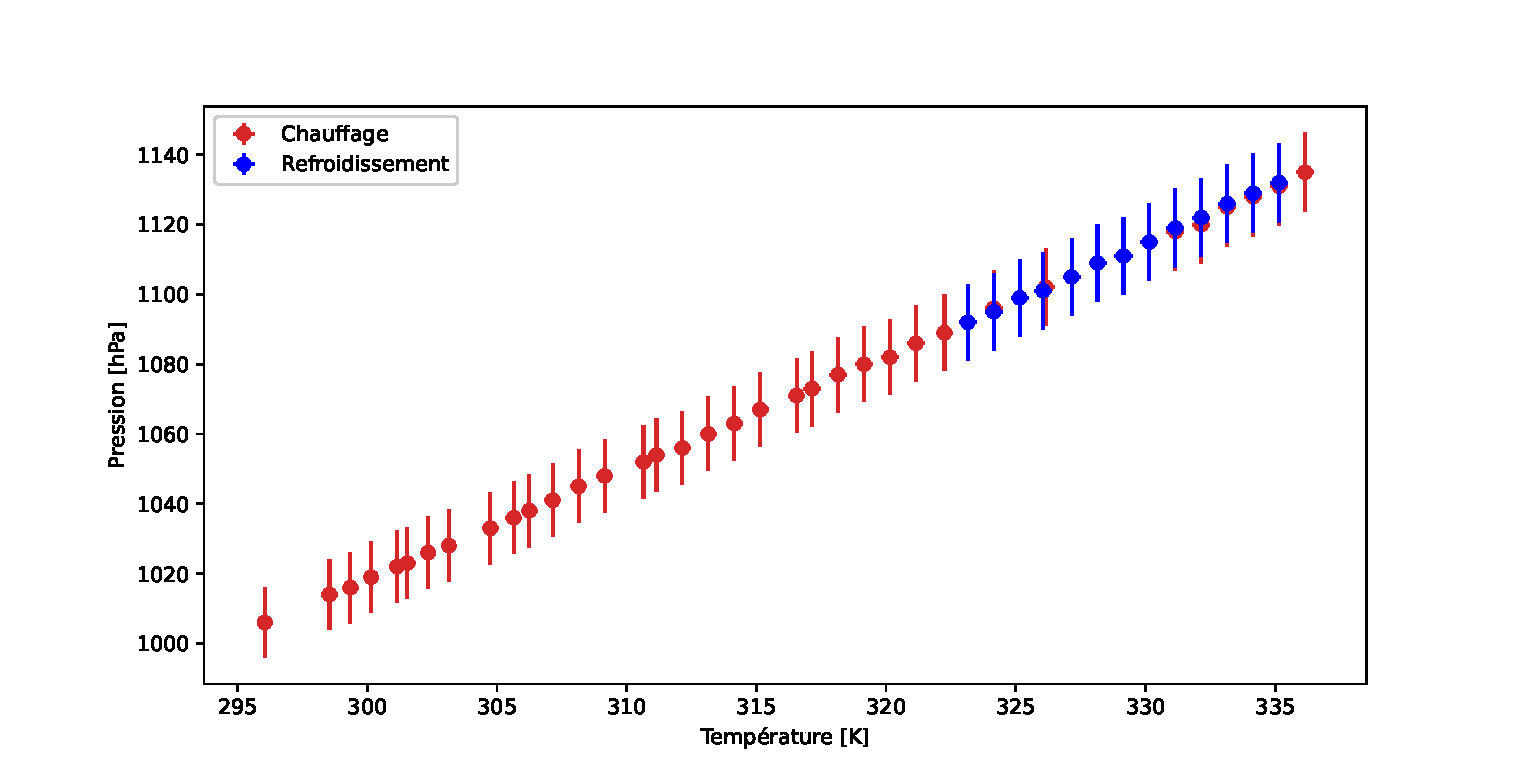
\includegraphics[scale=0.68]{img/exp2_graph1.eps}
		\caption{Pression $P$ en fonction de la température}
	\end{center}
	\label{Exp2_graph1}
\end{figure}

\textbf{Point sur les incertitudes:} nous avons relevé sur la fiche technique des appareils que l'incertitude était de 2\% (donc $\pm$ 1\%) de la valeur pour la pression, et 0.2\% (donc $\pm$ 0.1\%) pour la température, qu'on a donc représenté sur
le graphique.

Avant toute modélisation, on peut revenir sur la remarque précédente concernant la thermalisation de l'air de la bouteille. On note que les points de température et pression lors du chauffage et 
du refroidissement suivent la même tendance, ainsi que les mêmes valeurs. On en conclut donc par rapport à notre raisonnement précédent qu'il y avait bien thermalisation entre l'eau et l'air lors du chauffage.

\newpage
Pour déterminer le caractère linéaire de nos mesures, on réalise une régression linéaire de ces dernières et l'on compare au coefficient de corrélation. 
\begin{figure}[!h]
	\begin{center}
		\includegraphics[scale=0.65]{img/exp2_graph2.eps}
		\caption{Ajustement des mesures par un modèle linéaire de type $y=ax+b$}
	\end{center}
	\label{Exp2_graph2}
\end{figure}

On obtient un coefficient de corrélation $R^2 = 0.99984$, ce qui permet de conclure que nos mesures se comportent de façon très étroite et proche d'une fonction linéaire. On obtient donc les paramètres suivants:
\begin{align*}
	a = 3.21 \pm 0.14 hPa.K^{-1} \quad \quad b = 57 \pm 45 hPa
\end{align*}
\begin{equation*}
	P_{fit} = a * T + b
\end{equation*}

En reprendant la loi des gaz parfaits, cette dernière prédit qu'à $P = 0Pa$, la température doit être nulle, ou inversement lorsque $T = 0K$, on doit avoir $P=0Pa$. On peut donc vérifier cela
en extrapolant nos mesures. On peut déjà s'attendre à une valeur non nulle car l'ordonnée à l'origine $b$ ne l'est pas. On note $T_0$, la température à $P=0Pa$:

\begin{equation}
	T_0 = \frac{-b}{a}
\end{equation}

On en déduit l'incertitude associée :
\begin{equation}
	\delta T_0 = \frac{\delta b}{a} + \frac{b}{a^2} \delta a
\end{equation}

\newpage
Pour conclure cette expérience, nous avons obtenu un comportement linéaire de la pression en fonction de la température à volume constant pour des pressions proches de la pression atmosphérique.
Cependant, en prolongeant la régression linéaire de nos mesures, on obtient une température $T_0 = -18 \pm 15 K$ à $P=0Pa$, donc au plus proche de $0K$, $T_0 = -3K$, on note donc un écart à la théorie.
De plus, une température inférieure à $0K$ est impossible, le résultat est donc incohérent. Ce résultat peut potentiellement provenir de notre hypothèse de départ, c'est-à-dire que l'air est un gaz parfait. 
La littérature scientifique conclut que l'air est un gaz parfait pour des pressions proches de la pression atmosphérique, ce qui explique le bon comportement
de nos mesures avec la théorie. Cependant, il est possible que l'air ne suit plus un comportement de gaz parfait à des pressions quasi-nulles, ce qui semble être l'hypothèse la plus probable. 
Pour vérifier cette hypothèse, il serait possible de réaliser cette expérience dans une enceinte à vide pour la vérifier. 

\end{document}
